In this section, we will concentrate on the benchmarks and the more quantifiable outcomes of the project. The tests were conducted on a PC equipped with the following specifications:

\begin{itemize}
  \item CPU: Intel i5-4590, Threads: 4, Cores: 4, 3.7GHz
  \item RAM: 24GB DDR3
  \item OS: Zorin 16.2 (Ubuntu based)
\end{itemize}

To begin, let's examine \autoref{fig:pillar-plot}.

\begin{figure}[hbtp]
	\centering
	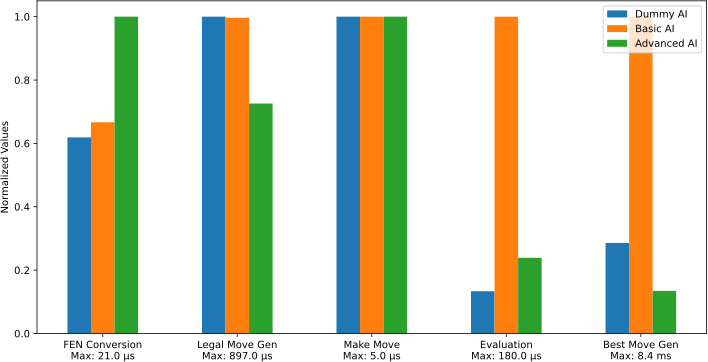
\includegraphics[width=.9\linewidth, page=1]{reference/pics/plot.pdf}
	\caption{Benchmarks of the different categories across the AI versions.}
	\label{fig:pillar-plot}
\end{figure}

The results are divided into five categories, with the first three determined by the chess backend and the latter two by the AI. It's important to note the significance of the legal move generation in the backend benchmarks. As the main bottleneck of the backend, any performance improvement in this area has a substantial impact on the overall performance of the AI. The reduction in time can be attributed to the refactoring process, which involved using lists of integers and minimizing boilerplate\footnote{
The Fen conversion is only used for debugging
purposes, the fact that it increased is not noticeable
in an optimized AI that doesn't debug anything.} code.

However, the most critical category is the final one, \textit{Best Move Generation}. As the name implies, this measures the speed at which the AI calculates the best move, in this case at a depth of one. Despite a slower evaluation compared to the previous version, the optimized AI demonstrates the best overall time. This underscores the fact that the final performance and strength of an AI are determined by multiple factors. In this instance, the number of nodes searched was significantly reduced by the implemented AI features, leading to an overall performance improvement.

This brings us to \autoref{fig:depth-plot}, which illustrates the relationship between time and the number of nodes searched in relation to the depths. As shown in the lower plot, the number of nodes searched is significantly lower for the optimized AI compared to the advanced AI\footnote{
The apparent lower number of nodes searched by the dummy and basic AI can be attributed to a bug in the early implementations of the AI related to move ordering. This issue was resolved in the third milestone. Therefore, the benchmarks for the dummy and basic AI in relation to depth should be interpreted with caution.
}. It's important to note that the apparent lower number of nodes searched by the dummy and basic AI is due to a bug in the early implementations of the AI related to move ordering, which was fixed in the third milestone. Therefore, the benchmarks for the dummy and basic AI in relation to depth should be interpreted with caution.

The plot also shows that the overall time is shorter for the optimized AI, regardless of depth. However, this is not always the case. For instance, if we had made poor decisions regarding the balance of exploration and exploitation in the MCTS, the performance could have actually been slower at higher depths. This highlights the importance of regular or atomic benchmarks, where a single element is changed to observe the system's response. Research also played a crucial role in fine-tuning the system.

\begin{figure}[hbtp]
	\centering
	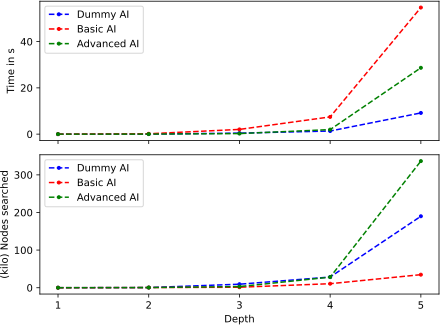
\includegraphics[width=.8\linewidth, page=1]{reference/pics/plot-depths.pdf}
	\captionsetup{justification=centering}
	\caption{Benchmarks of different AI versions in respect to search depth.\\Note that the number of nodes searched is in thousands (kilo).}
	\label{fig:depth-plot}
\end{figure}

\pagebreak
